\documentclass{article}
\usepackage[utf8]{inputenc}

\documentclass[a4paper]{article}
\usepackage[12pt]{extsizes}
\usepackage{amsthm, amssymb, amsmath, amsfonts, nccmath, empheq}
\usepackage{float}
\usepackage[hidelinks]{hyperref} 
\usepackage{color,colortbl} 
\renewcommand{\labelenumii}{\Roman{enumii}}
\usepackage[warn]{mathtext}
\usepackage[T1,T2A]{fontenc}
\usepackage[utf8]{inputenc}
\usepackage[english,russian]{babel}
\usepackage{tocloft}
\linespread{1.5}
\usepackage{indentfirst}
\usepackage{setspace}
%\полуторный интервал
\onehalfspacing


\newtheorem{theorem}{Теорема}
\newtheorem{definition}{Опредление}
\newtheorem{corollary}{Следствие}[theorem]
\newtheorem{lemma}{Лемма}


\newcommand{\RomanNumeralCaps}[1]
    {\MakeUppercase{\romannumeral #1}}

\usepackage{amssymb}

\usepackage{graphicx, float}
\graphicspath{{pictures/}}
\DeclareGraphicsExtensions{.pdf,.png,.jpg}
\usepackage[left=20mm,right=1cm,
    top=2cm,bottom=20mm,bindingoffset=0cm]{geometry}
\renewcommand{\cftsecleader}{\cftdotfill{\cftdotsep}}

\addto\captionsrussian{\renewcommand{\contentsname}{СОДЕРЖАНИЕ}}

\usepackage{fancyhdr}
\usepackage[nottoc]{tocbibind}

\fancypagestyle{plain}{%
\fancyhf{}
\renewcommand{\headrulewidth}{0pt}
\fancyhead[R]{\thepage}
}

\usepackage{blindtext}
\pagestyle{myheadings}
% href
\usepackage{hyperref}
\setcounter{MaxMatrixCols}{20}





\begin{document}
\begin{titlepage}
  \begin{center}
  
     
    \large
    
    Санкт-Петербургский политехнический университет Петра Великого
    
    Институт прикладной математики и механики
    
    \textbf{Высшая школа прикладной математики и вычислительной физики}
    
    \vfill
     
     
    \textsc{\textbf{\Large{Лабораторная работа №4}}}\\[5mm]
     
    {\large \textbf{Тема: <<Решение задач многомерной  минимизации без ограничений>>}}
    
    \\ по дисциплине\\ <<Методы оптимизаций>>\\

\end{center}

\vfill


\begin{tabular}{l p{140} l}
Выполнили студенты \\группы 3630102/80401   

&  &Мамаева Анастасия Сергеевна\\
&  &Веденичев Дмитрий Александрович\\
&  &Тырыкин Ярослав Алексеевич\\

Руководитель\\Доцент, к.ф.-м.н.& \hspace{0pt} &   Родионова Елена Александровна \\\\
\end{tabular}

\hfill \break
\hfill \break
\begin{center} Санкт-Петербург \\2021 \end{center}
\thispagestyle{empty}
 
\end{titlepage}
\newpage
\begin{center}
    \setcounter{page}{2}
    \tableofcontents  
\end{center}

\newpage
\section{Постановка задачи}
\noindent Пусть имеется задача многомерной минимизации :
$$f(x)=2x_1^{2}+x_2^{2}+cos(6x_1+5x_2)-x_1+2x_2 \longrightarrow \min_x$$
Необходимо:
\begin{enumerate}
    \item Решить данную задачу градиентным методом наискорейшего спуска с шагом по методу золотого сечения.
    \item Обосновать выбор условия окончания вычислений для метода одномерной минимизации по соответствующему условию градиентного метода. Показать справедливость своего вывода в ходе вычислительного эксперимента (для точности градиентного метода 0,01).
    \item Решить данную задачу методом Ньютона с постоянным шагом.
    \item Решить данную задачу методом Бройдена — Флетчера — Гольдфарба — Шанно с постоянным шагом.
    \item Выполнить сравнительный анализ алгоритмов методов.
    \item Нарисовать линии уровня функции цели и показать в ходе вычислительного эксперимента ортогональность звеньев градиентной ломаной для метода наискорейшего спуска.
\end{enumerate}

\section{Применимость методов}
\noindent Алгоритмы безусловной минимизации делятся на классы, в зависимости от порядка привлекаемых производных:
\begin{itemize}
    \item Нулевого порядка -- без привлечения производных
    \item Первого порядка -- с вычислением первой производной\\
    \dots
    \item $p$--ого порядка - вычисление производных $p$--ого порядка
\end{itemize}
В рамках нашего курса остановимся на методах первого и второго порядков.
Для того, чтобы градиентный метод наискорейшего спуска сходился, необходимо выполнение следующей теоремы:
\begin{theorem}
Если $f(x)$-- дифференцируемая функция, ограниченная снизу, её градиент удовлетворяет условию Липшица
$$||\nabla f(x) - \nabla f(y)|| \le R ||x-y||, ~~R>0$$
то будет выполняться $||\nabla f(x_k)|| \longrightarrow 0$ при $k \rightarrow \infty$  при любой начальной точке $x_0$.
\end{theorem}

\begin{theorem}
Если кроме того, функция $f(x)$ дважды непрерывно дифференцируема и существуют такие числа $0 < m \le M$, что
$$m||x||^{2}\le x^{T}H(y)x\le M||x||^{2},~~\forall~x,y$$
тогда $x_k \longrightarrow x^{*},~~ f(x_k) \longrightarrow f(x^{*})$ при любой начальной точке $x_0$.
\end{theorem}

\noindent Существует аналогичная теорема о сходимости методов второго порядка. Единственное отличие в том, что сходиться алгоритм будет со сверхлинейной скоростью.\\

\noindent С помощью пакета MATLAB2020b построим график функции:
\\
\begin{figure}[H]
\center{\includegraphics[scale=0.37]{Mo.jpg}}
\label{fig:image}
\end{figure}

\begin{figure}[H]
\center{\includegraphics[scale=0.57]{lines.png}}
\label{fig:image}
\end{figure}
\noindent Видим, что у нас неупорядоченный тип рельефа, в котором имеется несколько минимумов.

\begin{figure}[H]
\center{\includegraphics[scale=0.29]{5.jpg}}
\label{fig:image}
\end{figure}

\begin{figure}[H]
\center{\includegraphics[scale=0.87]{MO4_2.jpg}}
\label{fig:image}
\end{figure}

\begin{figure}[H]
\center{\includegraphics[scale=0.87]{MO4_3.jpg}}
\label{fig:image}
\end{figure}

\section{Описание алгоритмов}
\subsection{Градиентный метод наискорейшего шага}
\begin{enumerate}
    \item Начальный этап:
        \begin{enumerate}
             \item Выберем $\varepsilon>0,~~0<\alpha_0<1,~~x_0$ -- начальное приближение
             \item Положим $k=0$
        \end{enumerate}
    \item Основной этап:
        \begin{enumerate}
            \item Вычисляем $\nabla f(x_k),~~\alpha_k=\alpha_0$
            \item Подбор шага осуществляем наилучшим способом, то есть так, чтобы минимизировать разность между значением функции в следующей точке и значением функции в предыдущей точке:  $min f(x_k-\alpha_k \nabla f(x_k)),~~0<\alpha_k<1$\\
            Для решения этой задачи можем использовать любой метод одномерной минимизации.
            \item Полагаем $x_{k+1}=x_k-\alpha_k \nabla f(x_k)$, заменяем $k$ на $k+1$, переходим к шагу 2.\RomanNumeralCaps{1}
        \end{enumerate}
    \item Условие окончания вычислений:  $||\nabla f(x_k)||<\varepsilon$
\end{enumerate} 

\noindent В данном алгоритме есть необходимость использования одномерной минимизации, для поиска подходящего $\alpha_k$. Для этого воспользуемся методом золотого сечения.

\subsection{Метод золотого сечения}
\begin{enumerate}
    \item Найдём $x_1=a+\frac{3-\sqrt{5}}{2}(b-a),~~x_2=a+\frac{\sqrt{5}-1}{2}(b-a)$. Вычислим $f(x_1)~и~f(x_2)$. Положим $\tau=\frac{\sqrt{5}-1}{2},~~\varepsilon_n=b-a$.
    \item Проверка на окончание поиска: если $\varepsilon_n>\varepsilon$, то перейдём к шагу 3, иначе -- к шагу 4.
    \item Переходим к новому отрезку и новым пробным точкам. Если $f(x_1)\le f(x_2)$, то положим $b=x_2,~x_2=x_1,~f(x_2)=f(x_1),~x_1=b-\tau (b-a)$ и вычислим $f(x_1)$, иначе -- положим $a=x_1,~x_1=x_2,~f(x_1)=f(x_2),~ x_2=a+\tau (b-a)$ и вычислим $f(x_2)$. \\
    Положим $\varepsilon_n=\tau \varepsilon_n$ и перейдём к шагу 2.
    \item Окончание поиска: $x^{*}=\frac{a+b}{2},~f^{*}=f(x^{*})$
\end{enumerate}

\subsection{Метод Ньютона с постоянным шагом}
\begin{enumerate}
    \item Задаём начальное приближение $x_0$ и точность вычислений $\varepsilon>0$
    \item Вычисляем градиент рассматриваемой функции и квадратной матрицы Гессе:\\\\
    градиент рассматриваемой функции:
    \begin{equation*}
        \nabla f(x_k)=
        \begin{bmatrix}
        \frac{\partial}{\partial x_1} f(x_1, \dots ,x_n)\\
        \vdots\\
        \frac{\partial}{\partial x_n} f(x_1, \dots ,x_n)\\
        \end{bmatrix}
    \end{equation*}
    \\
    квадратная матрица Гессе:
    \begin{equation*}
        H(x_k)=\nabla^{2}f(x_k)=
        \begin{bmatrix}
        \frac{\partial^{2}}{\partial^{2} x_1} f(x_1, \dots ,x_n) & \dots &  \frac{\partial^{2}}{\partial x_1 \partial x_n} f(x_1, \dots ,x_n)\\
        \vdots & \ddots &  \vdots\\
        \frac{\partial^{2}}{\partial x_1 \partial x_n} f(x_1, \dots ,x_n) & \dots &
         \frac{\partial^{2}}{\partial^{2} x_n} f(x_1, \dots ,x_n)
        \end{bmatrix}
    \end{equation*}
    \item Определяем новые значения аргументов функции после выполнения $k-$ого шага расчёта методом по следующей формуле: $x_{k+1} =x_k - H^{-1}(x_k) \nabla f(x_k)$
    \item Условие окончаний вычислений: $||\nabla f(x_k)||<\varepsilon$. Если заданная точность не достигнута, то возвращаемся к шагу 3.
\end{enumerate}

\subsection{Метод Бройдена — Флетчера — Гольдфарба — Шанно с постоянным шагом}
\begin{enumerate}
    \item Задаём начальное приближение $\varepsilon$. Выбираем начальную точку $x_0$. Полагаем $A_1=E$ и строим множество $I_0=\{n,2n,\dots\}$ моментов обновления алгоритма. Полагаем $k=1$ и вычисляем $\omega_1=-\nabla f(x_0)$.
    \item На $k$--ом шаге проверяем выполнение неравенства: $||\omega_k||<\varepsilon$. Если оно выполняется, то итерации прекращаются, $x^{*}=x_{k-1},~f(x^{*})=f(x_{k-1})$, иначе переходим к третьему пунтку.
    \item Вычисляем направление спуска $p_k=A_k \omega_k$, шаг $\alpha_k: min \psi_k(\alpha)=f(x_{k-1}+\alpha p_k)$ и точку $x_k=x_{k-1}+\alpha_k p_k$. Вычисляем $\omega_{k+1}=-\nabla f(x_k)$. Если $k \in I_0$, то $A_{k+1}=E,~k=k+1$ и возвращаемся к пункту 2. Иначе -- переходим к пункту 4.
    \item Полагаем $\Delta x_k=x_k-x_{k-1}$, $\Delta \omega_k=\omega_k_+_1-\omega_k$, вычисляем матрицу $A_{k+1}$, $k=k+1$ и возвращаемся к пункту 2.
    Матрицу $A_{k+1}$ вычисляем по формуле:
    $$A_{k+1}=A_k-\frac{\Delta x_k(\Delta x_k)^T}{\Delta \omega_k^T \Delta x_k}-\frac{A_k \Delta \omega_k (\Delta \omega_k)^T A_k^T}{\Delta \omega_k^T A_k \Delta \omega_k}+\Delta \omega_k^T A_k \Delta \omega_k r^k (r^k)^T$$
    где $$r^k=\frac{A_k \Delta \omega_k}{ \Delta \omega_k^T A_k \Delta \omega_k}-\frac{\Delta x_k}{\Delta x_k^T \Delta \omega_k},~~~k \in \mathbb{N}$$
\end{enumerate}

\section{Результаты решения задачи}
\subsection{Численное решение задачи}
\noindent Решение задачи методом наискорейшего спуска с точностью $\varepsilon = 10^{-3}$ и начальной точкой $[-2,~2.7]$: 
$$x_k~=~[0.2722,~-0.9582]$$
$$f(x_k)~=~-2.1221$$

\noindent Решение задачи методом Ньютона с точностью $\varepsilon = 10^{-3}$ и начальной точкой $[0.4,~0.4]$: 
$$x_k~=~[0.2729,~-0.9588]$$
$$f(x_k)~=~-2.1220$$

\noindent Решение задачи методом БФГШ с точностью $\varepsilon = 10^{-3}$ и начальной точкой $[2,~-2.7]$:
$$x_k~=~[0.2727,~-0.9589]$$
$$f(x_k)~=~-2.1220$$

\subsection{Линии уровня, рельефы}
\noindent Все эффективные методы поиска минимума сводятся к построению траекторий, ыдоль которых функция убывает; разные методы отличаются способами построения таких траекторий. Метод, приспособленный к одному типу рельефа, может оказаться плохим на рельефе другого типа.\\\\
\noindent Линии уровня функции цели будут задаваться условием: $z=c$, то есть уравнениями вида $F(x,~y)=c$. Совокупность этих линий уровня для разных значений $c$ показывает рельеф функции. Построим линии уровня и покажем звенья ломаных поверх рельефа.

\begin{figure}[H]
\center{\includegraphics[scale=0.45]{eps_-1.jpg}}
\label{fig:image}
\end{figure}
\noindent Видим, что выполняется условие ортогональности звеньев, которое аналитически записывается в виде:
$$-\nabla^{T} f(x_{k+1})\nabla f(x_k)=0$$

\noindent Далее построим ломанную для метода Ньютона:
\begin{figure}[H]
\center{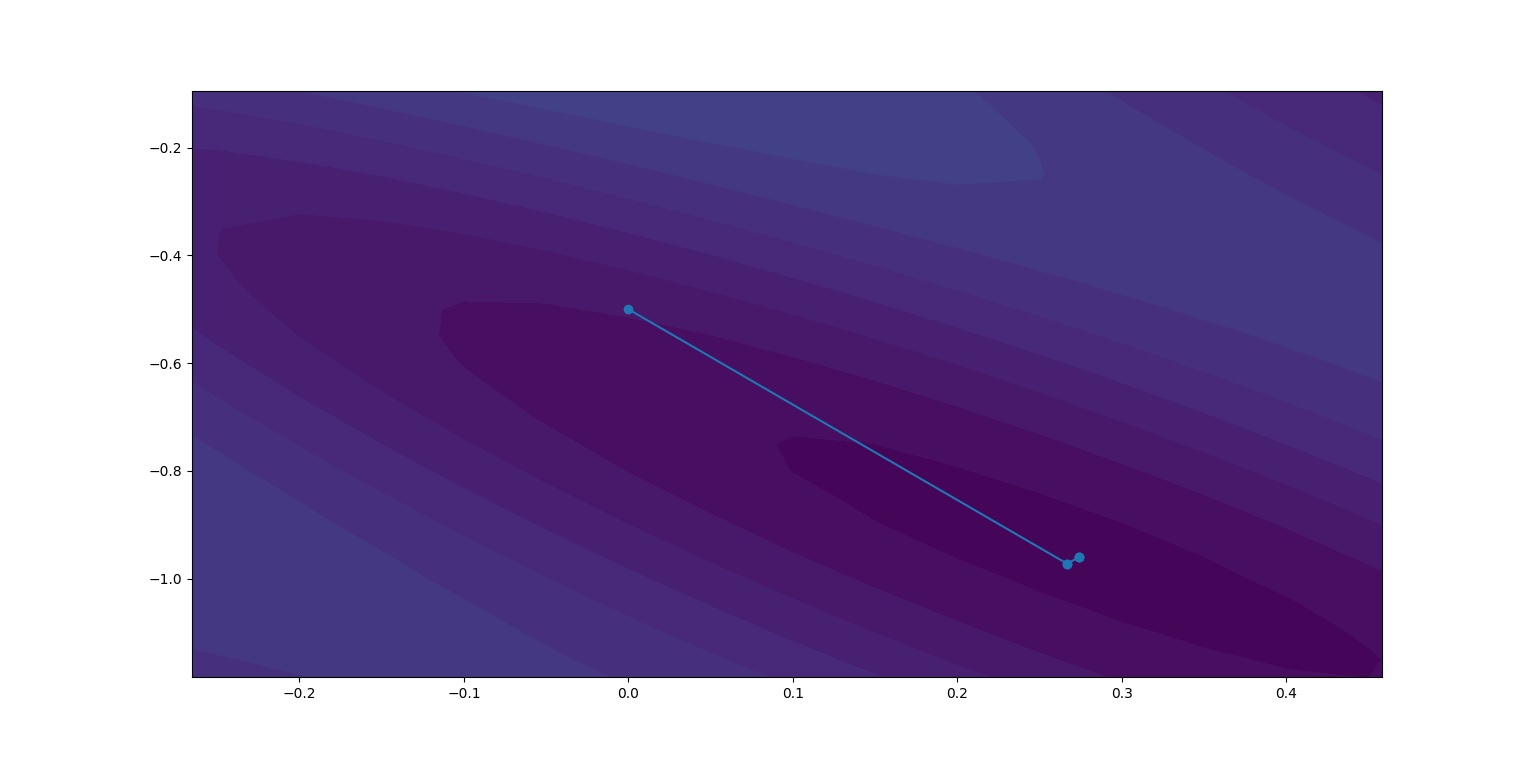
\includegraphics[scale=0.5]{Newton.jpeg}}
\label{fig:image}
\end{figure}
\noindent И для метода Бройдена — Флетчера — Гольдфарба — Шанно:
\begin{figure}[H]
\center{\includegraphics[scale=0.5]{BFGS_2.jpeg}}
\label{fig:image}
\end{figure}


\section{Сравнительный анализ}
\noindent Метод наискорейшего спуска гарантирует сходимость лишь в смысле $\lim_{k \to \infty}||\nabla f(x_k)||=0$, то есть сходимость по функции либо к точной нижней грани $inf f(x)$, либо к значению функции $f$ в некоторой  стационарной точке $x^{*}$. При этом сама точка $x^{*}$ не обязательно является точкой локального минимума; она может быть точкой седлового типа. Однако на практике подобная ситуация маловероятна и применение градиентных методов, как правило, позволяет получить приближенное значение минимума целевой функции (вообще говоря, локально).\\\\
\noindent Метод Ньютона по сравнению с градиентным состоит в том, что он <<не реагирует>> на овражный характер минимизируемой функции. Градиентные методы, по существу, используют линейную аппроксимацию целевой функции и поэтому менее точно определяют направление на точку минимума. Таким образом, метод Ньютона позволяет достигнуть заданной точности за меньшее число итераций, чем градиентные методы. Однако каждая итерация метода Ньютона связана с вычислением матрицы Гессе и последующим обращением, что требует большего объёма вычислений по сравнению с одной итерацией градиентного метода. Если начальная точка выбрана не достаточно близко к оптимальной, то с большой вероятностью метод разойдётся.
\\\\
\noindent Стремление уменьшить объем вычислений привело к созданию класса методов, близких по скорости сходимости к методу Ньютона, но не использующих вторые производные целевой функции $f(x)$ и процедуры обращения матрицы $f''(x)$. Недостатком этих методов является необходимость хранения в памяти ЭВМ матриц $A_k$, что при решении задач высокой размерности может создать определённые трудности.

\section{Проведение сравнительных экспериментов}
\noindent Ранее мы уже убедились, что наша фунция имеет несколько минимумов. Такое поведение характерно для квазивыпуклых функций. В связи с этим возникает желание провести эксперименты и понаблюдать, с какой скоростью будут сходиться методы, а также сравнить число итераций.
\begin{figure}[H]
\center{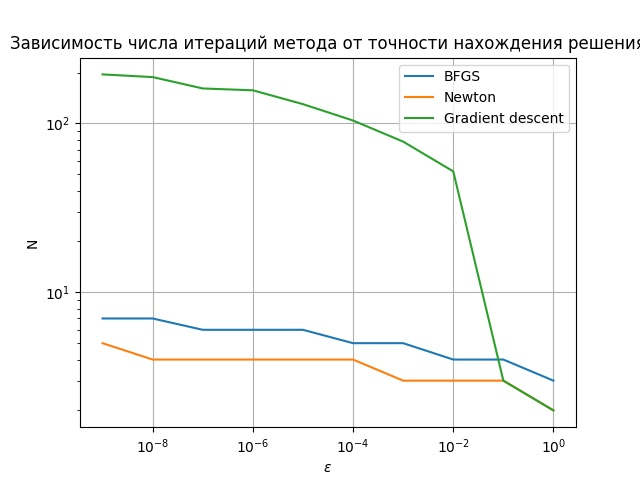
\includegraphics[scale=0.8]{Итерации.jpeg}}
\label{fig:image}
\end{figure}
\begin{figure}[H]
\center{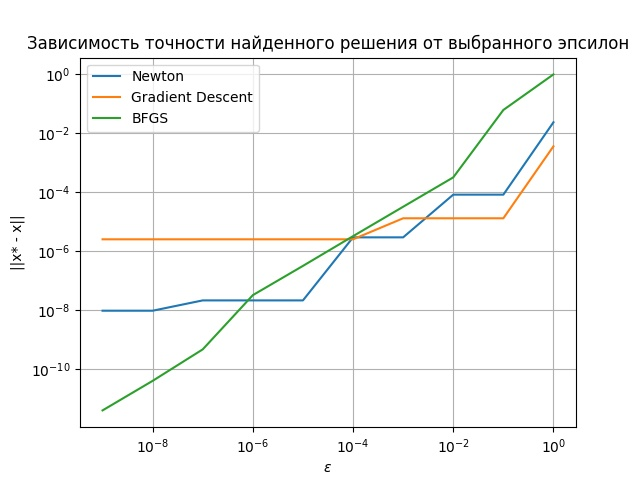
\includegraphics[scale=0.8]{Точность.jpeg}}
\label{fig:image}
\end{figure}
\noindent Видим, что для нашей функции  оптимальным является использование метода БФГШ.

\section{Оценка достоверности полученного результата}
\begin{figure}[H]
\center{\includegraphics[scale=0.5]{V.jpg}}
\label{fig:image}
\end{figure}

\section{Дополнительные исследования}
\subsection{Уточняющие детали градиентного спуска}
\noindent При поиске шага ставится задача: выйдя из точки $x_k$, найти в направлении антиградиента $-\nabla f(x_k)$ точку, дающую минимум функции $f(x_k - \alpha \nabla f(x_k))$. Пусть мы находимся в точке $x_k$ и выбираем шаг $\alpha_k$. Если $m$ -- наименьшее собсвтенное число Гессиана, то ближайший локальный минимум не может быть ближе к $x_k$, чем $\frac{||\nabla f(x_k)||}{m}$. Будем искать шаг на промежутке $\alpha = [\frac{1}{m},~1]$.
\\\\
\noindent Длина желаемого интервала неопределённости, до которого нужно сузить начальный, должна быть такой, чтобы в итоге достичь условия 
$$||\nabla f(x_k)||< \varepsilon, ~~k \rightarrow \infty$$
для этого достаточно локализовать точку минимума $x_k^{*}$ одномерной функции с точностью $\frac{\varepsilon}{R}$, где $R$ -- константа Липшица. Такой выбор позволяет, двигаясь в направлении точки с $\nabla f = 0$, гарантированно попасть в $x_k_+_1$ такую, что условие малости нормы градиента будет выполняться.

\subsection{Вариативность условия остановки методов}
\noindent В наших алгоритмах мы использовали $$||\nabla f||<\varepsilon$$ как условие остановки итерационных процессов. Однако может быть использовано равносильное ему $$||\nabla f||^{2}<\bar \varepsilon,~ где ~ \bar \varepsilon = \varepsilon^{2}$$ Но как понять, когда лучше использовать то или иное условие?\\\\
\noindent Из курса функционального анализа известно, что в конечномерных пространствах любые две нормы эквивалентны. Так, если выбрана первая $||\overrightarrow{x}||_{1}=\sum\limits_{k=1}^n x_k$ или бесконечная норма $||\overrightarrow{x}||_{\infty}=\max x_k$, то для упрощения вычислений легче воспользоваться критерием $||\nabla f||<\varepsilon$. Если мы работаем со второй нормой $||\overrightarrow{x}||_{2}=\sqrt{\sum\limits_{k=1}^n x_k^{2}}$ то с точки зрения вычислений проще воспользоваться критерием $||\nabla f||^{2}<\bar \varepsilon$. 
\\\\
Евклидова норма является геометрическим расстоянием между двумя точками в многомерном пространстве, поэтому целесеобразнее всего в работе было использовать её. В соответсвие с этим, во всех вышеописанных алгоритмах был подправлен критерий останова.

\section{Программная реализация}
\noindent В процессе реализации алгоритмов использовался язык программирования Python3.6. Для проверки полученных решений пользовались пакетом MATLAB2020b.
\\\\
\noindent Исходный код находится в системе контроля версий GitHub 
\\
https://github.com/Brightest-Sunshine/Optimization-methods-2021

\begin{thebibliography}{9}
\bibitem{book1} Лесин В. В., Лисовец Ю. П. Основы методов оптимизации: Учебное пособие. 3-е изд., испр, -- СПб.: Издательство <<Лань>>, 2011. -- 352с.
\bibitem{book2} Сухарев А. Г, Тимохов А. В., Фёдоров В. В Курс методов оптимизации: Учебное пособие, 2-е издание, -- М.:ФИЗМАТЛИБ, 2005, -- 368с.
\bibitem{book3} Ногин В. Д., Протодьяконов И. О., Еврампиев И. И. Основы теории оптимизации : Учебное пособие для вузов
\end{thebibliography}

\end{document}
